\documentclass[10pt]{standalone}
\usepackage[utf8]{inputenc}
\usepackage{pgfplots}
\pgfplotsset{compat=1.15}
\usepackage{mathrsfs}
\usepackage{amsmath}
\usetikzlibrary{arrows}
\pagestyle{empty}
\newcommand{\degre}{\ensuremath{^\circ}}
\begin{document}

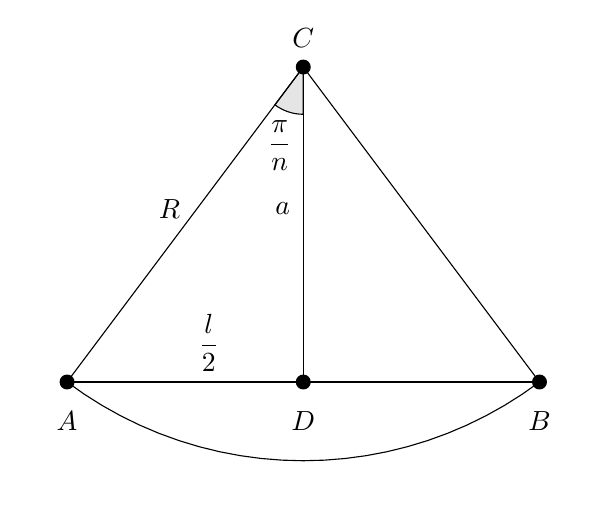
\begin{tikzpicture}[line cap=round,line join=round,>=triangle 45,x=1.0cm,y=1.0cm]
\clip(1.5,-0.5) rectangle (8.5,5.5);
\draw [shift={(5.,5.)},color=black,fill=black,fill opacity=0.10000000149011612] (0,0) -- (-126.86989764584402:0.6) arc (-126.86989764584402:-90.:0.6) -- cycle;
\draw  (2.,1.)-- (8.,1.);
\draw  (8.,1.)-- (5.,5.);
\draw  (5.,5.)-- (2.,1.);
\draw  (5.,5.)-- (5.,1.);
\draw [shift={(5.,5.)}]  plot[domain=4.068887871591405:5.355890089177974,variable=\t]({1.*5.*cos(\t r)+0.*5.*sin(\t r)},{0.*5.*cos(\t r)+1.*5.*sin(\t r)});

\draw [fill=black] (2.,1.) circle (2.5pt);
\draw[color=black] (2.,0.5) node {$A$};
\draw [fill=black] (8.,1.) circle (2.5pt);
\draw[color=black] (8.,0.5) node {$B$};
\draw [fill=black] (5.,5.) circle (2.5pt);
\draw[color=black] (5.0,5.37) node {$C$};
\draw[color=black] (3.8,1.5) node {$\dfrac{l}{2}$};
%\draw[color=black] (6.8,3.37) node {$g$};
\draw[color=black] (3.3,3.2) node {$R$};
\draw [fill=black] (5.,1.) circle (2.5pt);
\draw[color=black] (5.,0.5) node {$D$};
\draw[color=black] (4.74,3.2) node {$a$};
%\draw[color=black] (5.16,0.31) node {$c$};
\draw[color=black] (4.7,4.0) node {$\dfrac{\pi}{n}$};

\end{tikzpicture}
\end{document}